\documentclass{article}

\usepackage{tikz}
\usepackage{xcolor}

\usetikzlibrary{
  positioning,
  calc,
  shapes.multipart,
  external,
  arrows.meta,
  fit
}

\tikzset{
  >=Triangle,
  n/.style = {
    circle, draw=black!30, line width=1pt
  },
  w/.style = {
    n, fill=green!10
  },
  pics/nnn/.style = {
    code = {
      \node [circle split, draw=black!30, line width=1pt, fill=blue!10] (-n) {
        $a$
        \nodepart{lower}
        $\sum$
      };
    }
  }
}

\tikzexternalize[prefix=figures/]

\begin{document}
% A single neural network neuron
\tikzsetnextfilename{nn-neuron}
\begin{center}
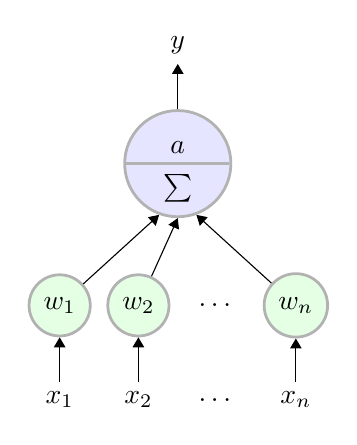
\begin{tikzpicture}
  \path
    (0,0) node [] (x1) {$x_1$}
    (1,0) node [] (x2) {$x_2$}
    (2,0) node [] {\ldots}
    (3,0) node [] (xn) {$x_n$}
    (0,1.2) node [w] (w1) {$w_1$}
      edge [<-] (x1)
    (1,1.2) node [w] (w2) {$w_2$}
      edge [<-] (x2)
    (2,1.2) node [] {\ldots}
    (3,1.2) node [w] (wn) {$w_n$}
      edge [<-] (xn)
    (1.5,3) pic [] (nnn) {nnn}
      (nnn-n.250) edge [<-] (w1)
      (nnn-n.270) edge [<-] (w2)
      (nnn-n.290) edge [<-] (wn)
    (1.5,4.5) node [] {$y$}
      edge [<-] (nnn-n.north);
\end{tikzpicture}
\end{center}
\end{document}